\documentclass[11pt]{article}
\usepackage[margin=1in]{geometry}
\usepackage{amsmath,amssymb,amsthm}
\usepackage{booktabs}
\usepackage{graphicx}
\usepackage{hyperref}
\usepackage{xcolor}
\usepackage{caption}
\usepackage{enumitem}

\newcommand{\R}{\mathbb{R}}
\newcommand{\E}{\mathcal{E}}
\newcommand{\V}{\mathcal{V}}
\newcommand{\N}{\mathcal{N}}
\DeclareMathOperator*{\argmin}{arg\,min}

\title{GPU-Cluster Scheduling Fragmentation: Problem Formulation,\\
Algorithms, Stress-Test Scenarios, and Empirical Comparison}
\author{gputrace + py\_sim}
\date{Run \texttt{2026-09-12\_fgd\_vs\_wfgd\_htafm} \\ \small full manifest, seeds, and raw data in \texttt{experiments/runs/2026-09-12\_fgd\_vs\_wfgd\_htafm/}}

\begin{document}
\maketitle

\begin{abstract}
We formalize GPU-cluster scheduling as a constrained online bin-packing
problem, give precise mathematical definitions for thirteen scheduling
algorithms evaluated on a common test bed (eight node-granularity
heuristics, Fragmentation Gradient Descent \cite{fgd}, two new variants we
introduce -- \textsc{w-fgd} and \textsc{w-fgd-balanced} -- and three
variants of the topology-aware H-TAFM metric \cite{fgd,defrag,hypergraph_survey,partitioning_hard,binpacking_survey}),
formalize the statistical generation process behind fourteen synthetic
stress-test scenarios (\texttt{gputrace}), and report a full empirical
comparison across all thirteen algorithms and fourteen scenarios with
explicit significance tests. \textbf{Headline result}: \textsc{w-fgd-balanced}
significantly reduces rejection rate relative to plain FGD in batch/static
placement (Wilcoxon signed-rank $p=0.0035$, $n=14$ scenario blocks) and
significantly reduces SLA-violation rate in realistic time-driven operation
($p=0.037$), but is \emph{not} distinguishable from the strongest existing
simple heuristic, \textsc{least\_requested} ($p=0.81$) -- we report this
honestly rather than only the comparison that favors our contribution.
\end{abstract}

\tableofcontents

% =====================================================================
\section{Problem Formulation}
% =====================================================================

\subsection{Cluster model}
A cluster is a set of nodes $\N = \{n_1, \dots, n_M\}$. Each node $n_i$ has
a fixed capacity vector
\[
  c(n_i) = \big(c^{\text{cpu}}_i,\; c^{\text{gpu}}_i,\; c^{\text{mem}}_i\big) \in \R_{\geq0}^3,
\]
where $c^{\text{cpu}}_i$ is milli-CPU capacity, $c^{\text{gpu}}_i$ is GPU
count (an integer, treated as a set of $c^{\text{gpu}}_i$ homogeneous
1000-milli-GPU units within a node), and $c^{\text{mem}}_i$ is memory in
MiB (assumed, not tracked in the base schema -- \S\ref{sec:mem-assumption}).
Each node also has a categorical attribute $\tau(n_i) \in \{\text{V100},
\text{A100}, \text{T4}, \text{H100}, \dots\}$.

\subsection{Job (pod) model}
A job $p$ arrives at time $s(p) \geq 0$ (\emph{submit time}) with a resource
request vector
\[
  r(p) = \big(r^{\text{cpu}}(p),\; r^{\text{gpu}}(p),\; g(p)\big),
\]
a required GPU type $\tau(p)$ (or $\varnothing$ for CPU-only), a service
duration $d(p) > 0$, and a tenant/user label $u(p)$. A job is
\emph{feasible} on node $n_i$ at time $t$ iff every dimension of $n_i$'s
\emph{residual} capacity at $t$ dominates $r(p)$ and, if $\tau(p) \neq
\varnothing$, $\tau(p) = \tau(n_i)$:
\[
  \mathrm{fits}(p, n_i, t) \iff r^{\text{cpu}}(p) \leq \rho^{\text{cpu}}_i(t)
  \;\wedge\; r^{\text{gpu}}(p) \leq \rho^{\text{gpu}}_i(t)
  \;\wedge\; \big(\tau(p)=\varnothing \vee \tau(p)=\tau(n_i)\big).
\]

\subsection{Two operating modes}
We evaluate every algorithm in two modes, matched to two different
questions:

\begin{description}[leftmargin=1.2em]
\item[\textsc{static} (batch)] All $|P|$ jobs are placed in one pass, in a
  fixed order, against a cluster with no time dimension -- $s(p)$ and
  $d(p)$ are ignored entirely. This measures pure \emph{packing quality}: given
  a fixed offered load, how much of it can a placement policy admit onto
  fixed capacity? It is also the \emph{only} mode H-TAFM has (it is a
  one-shot, not time-driven, algorithm), so it is the mode in which all
  thirteen algorithms are directly comparable.
\item[\textsc{time-driven}] Jobs arrive at their real $s(p)$, occupy their
  node for $[t_{\text{start}}(p), t_{\text{start}}(p)+d(p))$, and release
  capacity on completion; jobs that cannot be placed immediately queue
  (optionally with a max wait time, unused here) rather than being rejected
  outright. This measures \emph{operational} behavior: queueing delay,
  throughput, and whether a policy's static-mode packing advantage
  survives contact with realistic arrival dynamics.
\end{description}

\subsection{Objective}
There is no single scalar objective in the literature this problem draws
from; we report multiple objectives explicitly rather than reducing to
one:
\[
  \text{rejection rate } = 1 - \frac{|\{p : \text{admitted}(p)\}|}{|P|},
  \qquad
  \text{fragmentation}(\N, t) = \frac{1}{M}\sum_{i=1}^M
  \mathbb{1}\!\left[\exists\, \hat p \in \hat P : \neg\,\mathrm{fits}(\hat p, n_i, t)\right],
\]
where $\hat P$ is a small set of \emph{representative} job shapes (\S\ref{sec:fgd}),
plus wait-time percentiles, an SLA-violation rate, a fairness index, and
GPU-hours wasted, all defined in \S\ref{sec:broader-metrics}.

\subsection{Assumptions}
\begin{enumerate}[leftmargin=1.4em]
  \item \textbf{No preemption of running jobs.} Once admitted, a job runs
    to completion (the \texttt{spot\_preemption\_churn} scenario models
    preemption as inflated \emph{duration}, not as a scheduler-visible
    event -- see \S\ref{sec:scenarios}).
  \item \textbf{Nodes are the atomic placement unit} for all
    node-granularity algorithms; a job cannot span multiple nodes.
    H-TAFM relaxes this to NUMA-vertex granularity (\S\ref{sec:htafm}),
    which is strictly finer, not coarser.
  \item \textbf{GPUs within a node are homogeneous and fungible.} A job
    requesting $k$ GPUs on an 8-GPU node can use any $k$ of the 8; there is
    no GPU-topology (NVLink/PCIe) affinity modeled at the node level.
  \item \textbf{Memory is assumed, not measured}, wherever it is used at
    all (\S\ref{sec:mem-assumption}) -- the base gputrace/k8s\_sim schema
    does not carry a real memory field.
  \item \textbf{Arrivals and job sizes are drawn from a fixed statistical
    model} fit once to a reference distribution (or a real trace, if
    supplied), not re-fit per scenario -- each scenario perturbs specific,
    named aspects of that model (\S\ref{sec:scenarios}), not everything at
    once.
\end{enumerate}

% =====================================================================
\section{Scheduling Algorithms}
% =====================================================================

Every algorithm below has the signature $\pi : (p, \{n_i\}, t) \mapsto
n^\star \in \{n_i\} \cup \{\bot\}$ (choose a feasible node, or refuse).

\subsection{Baseline node-granularity heuristics}
Let $F(p,t) = \{n_i \in \N : \mathrm{fits}(p, n_i, t)\}$.

\begin{align*}
  \pi_{\text{random}}(p,t) &= \text{Uniform}(F(p,t)) \\
  \pi_{\text{first\_fit}}(p,t) &= \min\big(F(p,t)\big) \quad\text{(by fixed node index order)} \\
  \pi_{\text{best\_fit}}(p,t) &= \argmin_{n \in F(p,t)} \; \rho^{\text{gpu}}(n,t) - r^{\text{gpu}}(p)
    \quad\text{(least leftover GPU capacity)} \\
  \pi_{\text{worst\_fit}}(p,t) &= \argmax_{n \in F(p,t)} \; \rho^{\text{gpu}}(n,t) - r^{\text{gpu}}(p)
    \quad\text{(most leftover)} \\
  \pi_{\text{round\_robin}}(p,t) &= \text{next feasible node in cyclic node order, stateful across calls} \\
  \pi_{\text{gpu\_packing}}(p,t) &= \argmin_{n \in F(p,t)} \; \rho^{\text{gpu}}(n,t)
    \quad\text{(consolidate onto already-busy nodes)} \\
  \pi_{\text{least\_requested}}(p,t) &= \argmax_{n \in F(p,t)} \; \rho^{\text{gpu}}(n,t)
    \quad\text{(spread load; Kubernetes' default-like heuristic)}
\end{align*}

\subsection{Fragmentation Gradient Descent (FGD)}
\label{sec:fgd}
FGD \cite{fgd} scores a placement not by raw leftover capacity but by how
many \emph{representative} job shapes $\hat P = \{\hat p_1, \dots, \hat
p_5\}$ could still be placed afterward. $\hat P$ is derived once per
workload by taking, independently per resource dimension, the
$\{10,30,50,70,90\}$-th percentiles:
\[
  \hat p_k = \Big(\text{Quantile}_{q_k}\big(r^{\text{cpu}}(P)\big),\;
                    \text{Quantile}_{q_k}\big(r^{\text{gpu}}(P)\big),\;
                    \text{Quantile}_{q_k}\big(g(P)\big)\Big), \quad q \in \{.1,.3,.5,.7,.9\}.
\]
The \emph{unfit fraction} of a node is
\[
  U(n,t) = \frac{1}{|\hat P|}\sum_{\hat p \in \hat P} \mathbb{1}[\neg\,\mathrm{fits}(\hat p, n, t)],
\]
and FGD places greedily on the node whose unfit fraction increases least:
\[
  \pi_{\text{fgd}}(p,t) = \argmin_{n \in F(p,t)} \Big[U\big(n, t \oplus p\big) - U(n,t)\Big],
\]
where $t \oplus p$ denotes the hypothetical state after placing $p$ on
$n$. If $F(p,t)=\varnothing$, refuse; if $\hat P$ is empty (no GPU jobs
seen), fall back to $\pi_{\text{best\_fit}}$.

\subsection{Two weaknesses in FGD's own definition}
\label{sec:fgd-weaknesses}
Two properties of $U$ above are checkable directly from its definition,
not assumptions:

\begin{enumerate}[leftmargin=1.4em]
\item \textbf{Uniform weighting.} $U$ is an unweighted mean over 5 shapes.
  A placement that blocks $\hat p_{.9}$ (rare, 10\% of demand mass by
  construction) costs FGD's gradient exactly as much as one blocking
  $\hat p_{.5}$ (the median, by far the more common case in practice) --
  the metric cannot express that these are not equally costly mistakes.
\item \textbf{Per-dimension (``chimera'') quantiles.} Each $\hat p_k$'s
  three coordinates are the $q_k$-quantile of each resource \emph{marginal
  distribution independently}. Unless CPU and GPU demand are perfectly
  rank-correlated (they are not, in every scenario we measured --
  \S\ref{sec:scenarios}), $\hat p_k$ is a coordinate combination that may
  not correspond to any job actually present in $P$.
\end{enumerate}

\subsection{\textsc{w-fgd} and \textsc{w-fgd-balanced}: our contribution}
\label{sec:wfgd}
We replace $\hat P$'s construction with a \emph{stratified, weighted,
joint-sample} procedure. Let $m(p) = \tilde r^{\text{cpu}}(p) + \tilde
r^{\text{gpu}}(p)$ be a normalized demand magnitude (each resource
divided by its population max). Sort $P$ by $m$ and split into $K=5$
equal-count strata $S_1,\dots,S_K$. For each stratum, take the
\emph{medoid} -- the real job whose magnitude is closest to the
stratum's median magnitude -- as the representative shape, with weight
equal to the stratum's population share:
\[
  \hat p_k = \argmin_{p \in S_k} \big| m(p) - \mathrm{median}(m(S_k)) \big|,
  \qquad
  w_k = \frac{|S_k|}{|P|}, \qquad \sum_k w_k = 1.
\]
This directly resolves both weaknesses in \S\ref{sec:fgd-weaknesses}: every
$\hat p_k$ is a real, observed job (fixes the chimera problem), and $w_k$
reflects actual population mass (fixes uniform weighting). The weighted
unfit fraction and greedy rule are
\[
  U_w(n,t) = \sum_{k} w_k\, \mathbb{1}[\neg\,\mathrm{fits}(\hat p_k, n, t)],
  \qquad
  \pi_{\text{w\_fgd}}(p,t) = \argmin_{n \in F(p,t)} \Big[U_w(n, t\oplus p) - U_w(n,t)\Big].
\]

\textsc{w-fgd-balanced} adds a slack-preservation regularizer: among
nodes close on the weighted-fragmentation delta, prefer leaving more nodes
completely empty (strictly more valuable, ex ante, for an unknown future
large job than the same idle capacity spread thin):
\[
  \pi_{\text{w\_fgd\_bal}}(p,t) = \argmin_{n \in F(p,t)}
  \Big[\underbrace{U_w(n,t\oplus p) - U_w(n,t)}_{\text{fragmentation cost}}
  \;+\; \lambda \underbrace{\;\phi^{\text{gpu}}(n, t\oplus p)\;}_{\text{post-placement GPU utilization}}\Big],
  \quad \lambda = 0.15,
\]
where $\phi^{\text{gpu}}(n,t) = 1 - \rho^{\text{gpu}}(n,t)/c^{\text{gpu}}(n)$.
$\lambda=0$ recovers \textsc{w-fgd} exactly (verified by test, \S\ref{sec:repro}).
$\lambda=0.15$ was chosen by a small grid search on the baseline scenario
trading off static-mode rejection against time-driven SLA-violation rate;
it is a hyperparameter, not a derived constant, and should be re-tuned for
workloads with a very different size distribution.

\subsection{H-TAFM: topology-aware, multi-resource fragmentation}
\label{sec:htafm}
H-TAFM \cite{fgd,defrag,hypergraph_survey,partitioning_hard,binpacking_survey}
generalizes FGD's node-level, GPU-only metric to a NUMA-vertex-level,
three-resource (CPU+Memory+GPU) hypergraph. Physical topology is modeled as
a hypergraph $H=(\V,\E)$: each node is split into $\sigma$ NUMA vertices
(default: 2 sockets $\times$ 1 NUMA region), and hyperedges group vertices
at socket, server (node), and rack granularity, each with a scalar weight
$w(e)$. A vertex $v$'s capacity/free vectors are 3-tuples
$(c^{\text{cpu}}_v, c^{\text{mem}}_v, c^{\text{gpu}}_v)$; the free vector
after hypothetically placing demand $d$ is $f(v) - d$ where $d =
(r^{\text{cpu}}, r^{\text{mem}}, g\cdot 1000)$.

Three variants of the per-edge fragmentation potential $\phi(e)$:

\paragraph{Cut ($\phi_{\text{cut}}$).} For a set of pending reference
demands $D$, an edge is fragmented iff the \emph{aggregate} free capacity
across its vertices could satisfy some $d \in D$, but \emph{no single
vertex} can -- capacity exists, split unusably:
\[
  F_e = \sum_{v \in e} f(v), \qquad
  \phi_{\text{cut}}(e, D) = \mathbb{1}\Big[\exists\, d \in D:\; d \preceq F_e \;\wedge\; \forall v \in e,\; d \not\preceq f(v)\Big].
\]

\paragraph{Entropy ($\phi_{\text{entropy}}$).} The Shannon entropy of the
normalized free-capacity distribution across an edge's vertices:
\[
  s_v = \sum_{k} \frac{f_k(v)}{c_k(v)}, \qquad
  \phi_{\text{entropy}}(e) = -\sum_{v \in e} \bar s_v \log \bar s_v, \quad \bar s_v = \frac{s_v}{\sum_{v' \in e} s_{v'}}.
\]
Note this is \emph{maximized}, not zero, on a uniform/empty cluster --
low entropy signals free capacity concentrated in few vertices
(informative fragmentation), not the absence of it.

\paragraph{Hierarchical ($\phi_{\text{hier}}$).} A vertex counts as
fragmented if \emph{any} resource dimension has fallen below a fraction
$\theta$ (default $0.5$) of that vertex's capacity:
\[
  \phi_{\text{hier}}(e) = \lambda_{\text{level}(e)} \cdot
  \frac{1}{|e|}\sum_{v \in e} \mathbb{1}\Big[\min_k \tfrac{f_k(v)}{c_k(v)} < \theta\Big].
\]

\paragraph{Aggregate and greedy placement.}
\[
  \mathrm{TAFI}(H) = \sum_{e \in \E} w(e)\,\phi(e), \qquad
  \Delta\mathrm{TAFI}(v, d) = \sum_{e \ni v} w(e)\big[\phi(e \mid v \oplus d) - \phi(e)\big],
\]
and the scheduler places each demand on $\argmin_v \Delta\mathrm{TAFI}(v,d)$
among feasible vertices, touching only the (few) hyperedges containing
$v$ -- $O(|\E_v|)$ per placement, not $O(|\E|)$.

\subsection{Memory: an explicit, labeled assumption}
\label{sec:mem-assumption}
Neither gputrace's export schema nor the base \texttt{k8s\_sim} node/pod
model carries a real memory field. Wherever H-TAFM (which is genuinely
3-resource) is run against gputrace-exported data, we assume
\[
  \text{memory}_{\text{MiB}} = 8 \times \text{milli-cpu}
\]
on \emph{both} node capacity and job demand -- the same ratio
\texttt{k8s\_sim.topology}'s own fallback already documents. This keeps
comparisons internally consistent but means H-TAFM's \emph{absolute}
numbers should not be read as memory-accurate; the relative comparison
across scenarios and algorithms is far less sensitive to this constant
than the absolute fragmentation values are.

% =====================================================================
\section{Stress-Test Scenario Generation}
\label{sec:scenarios}
% =====================================================================

\subsection{Base statistical model}
gputrace fits a reference workload (Alibaba \texttt{cluster-trace-gpu-v2020}
sample, or the user's own trace) to a small bank of candidate distributions
via MLE and selects by AIC. Duration is best fit by log-normal,
$d \sim \mathrm{LogNormal}(\mu, \sigma)$; CPU/GPU request magnitude by
Burr Type XII; inter-arrival time by a heavy-tailed distribution whose
best-AIC fit (Pareto, shape $<1$) has \emph{infinite theoretical mean} --
sampling from it directly for simulation is capped at $5\times$ the
empirical maximum gap rather than used unbounded, a distinction we flag
explicitly because best-AIC-fit is not the same property as
safe-to-extrapolate-from.

\subsection{Per-scenario statistics, this run}
\label{sec:scenario-stats}
Table~\ref{tab:scenario-stats} reports summary statistics computed
directly from the archived, seed-42, $n=300$-job-per-scenario data used
for every result in this document (\texttt{results/gputrace\_data\_statistics.csv}).

\begin{table}[h]
\centering
\caption{Per-scenario duration statistics (seed 42, $n=300$ jobs/scenario). CV = coefficient of variation.}
\label{tab:scenario-stats}
\small
\begin{tabular}{lrrrrr}
\toprule
scenario & mean dur. (s) & median dur. (s) & CV & skew & kurtosis \\
\midrule
baseline                  & 457.8 & 200.1 & 1.75 & 4.47 & 26.6 \\
bursty\_arrivals          & 363.5 & 174.1 & 2.12 & 8.68 & 102.9 \\
checkpoint\_io\_burst     & 488.1 & 229.3 & 1.64 & 4.47 & 26.7 \\
cold\_start\_storm        & 14.8  & 10.8  & 0.98 & 1.84 & 4.3 \\
diurnal\_pattern          & 500.1 & 177.6 & 2.05 & 5.48 & 38.6 \\
flash\_crowd              & 461.3 & 198.0 & 1.75 & 4.39 & 25.8 \\
gpu\_fragmentation\_sharing & 457.8 & 200.1 & 1.75 & 4.47 & 26.6 \\
heavy\_tail\_demand       & 457.8 & 200.1 & 1.75 & 4.47 & 26.6 \\
high\_contention          & 457.8 & 200.1 & 1.75 & 4.47 & 26.6 \\
llm\_inference\_bursty    & 1.9   & 1.4   & 0.97 & 2.56 & 10.9 \\
long\_context\_kv\_pressure & 838.8 & 237.6 & 2.20 & 5.47 & 42.0 \\
moe\_expert\_load\_skew   & 457.8 & 200.1 & 1.75 & 4.47 & 26.6 \\
resource\_starvation      & 457.8 & 200.1 & 1.75 & 4.47 & 26.6 \\
spot\_preemption\_churn   & 358.1 & 134.3 & 1.88 & 4.33 & 23.7 \\
\bottomrule
\end{tabular}
\end{table}

\subsection{An honest finding: which scenarios actually differ from baseline, and how}
Testing exact column-wise equality against \texttt{baseline} at this seed
(Table~\ref{tab:identity}) reveals a precise, checkable structure:

\begin{table}[h]
\centering
\caption{Which columns differ from \texttt{baseline}, this seed (\checkmark = identical to baseline).}
\label{tab:identity}
\small
\begin{tabular}{lcccc}
\toprule
scenario & GPU demand & CPU demand & duration & submit\_time \\
\midrule
heavy\_tail\_demand        & \checkmark & \checkmark & \checkmark & \checkmark \\
checkpoint\_io\_burst      & \checkmark & \checkmark &            & \checkmark \\
long\_context\_kv\_pressure & \checkmark & \checkmark &            & \checkmark \\
high\_contention           & \checkmark & \checkmark & \checkmark &            \\
moe\_expert\_load\_skew    & \checkmark & \checkmark & \checkmark &            \\
resource\_starvation       &            &            & \checkmark & \checkmark \\
gpu\_fragmentation\_sharing &           & \checkmark & \checkmark &            \\
spot\_preemption\_churn    & \checkmark & \checkmark &            &            \\
bursty\_arrivals, cold\_start\_storm, diurnal\_pattern, & & & & \\
\quad flash\_crowd, llm\_inference\_bursty & \multicolumn{4}{c}{differ in every column} \\
\bottomrule
\end{tabular}
\end{table}

Several of these are correct by design: \texttt{high\_contention} and
\texttt{moe\_expert\_load\_skew} are specified to act through GPU-type
distribution and arrival pattern respectively, not raw magnitude, so
identical GPU/CPU/duration columns are expected; \texttt{checkpoint\_io\_burst}
and \texttt{long\_context\_kv\_pressure} act through duration and
submit\_time-adjacent mechanisms. \textbf{One case is not obviously
correct by design}: \texttt{heavy\_tail\_demand} is identical to
\texttt{baseline} in \emph{every} column at this seed, including
submit\_time -- its own name and gputrace's documentation describe a
resource-\emph{size} change (a fatter Pareto tail on CPU/GPU demand) that
is not observed here. We report this as a discrepancy worth checking in
gputrace's \texttt{generators/stress\_scenarios.py} against its
documented design, not as a claim about py\_sim.

% =====================================================================
\section{Experimental Setup}
% =====================================================================
Cluster: 20 nodes $\times$ 8 GPUs $=160$ GPUs, mixed GPU types (A100/V100/T4/H100)
per gputrace's default k8s\_sim export. 300 jobs/scenario, 14 scenarios,
seed 42, gputrace reference fit (no real trace supplied for this run --
see Appendix / manifest). Static mode: 1 run per algorithm per scenario
(deterministic except \texttt{random}). Time-driven mode: 3 seeds
$\times$ 10 node-granularity algorithms $\times$ 14 scenarios $=420$ runs.
SLA threshold for violation-rate: 60s wait.

\subsection{Reproducibility}
\label{sec:repro}
Every number in this document is reproducible from
\texttt{experiments/runs/2026-09-12\_fgd\_vs\_wfgd\_htafm/}: \texttt{manifest.json}
records the exact gputrace commit, generation/export commands, seeds, and
cluster shape; \texttt{gputrace\_raw/} and \texttt{gputrace\_export/}
archive the actual generated data (so reproduction does not depend on
gputrace's scenario-generation logic being unchanged upstream);
\texttt{reproduce.sh} re-runs every sweep against that archived data in
one command. \texttt{results/} and \texttt{plots/} hold the exact outputs
this document reports.

% =====================================================================
\section{Broader Evaluation Metrics}
\label{sec:broader-metrics}
% =====================================================================
Beyond rejection rate and mean wait time, we report:

\begin{align*}
  \text{Jain's Fairness Index \cite{jain1984}:} \quad & J(x_1,\dots,x_n) = \frac{\big(\sum_i x_i\big)^2}{n \sum_i x_i^2} \in \big(\tfrac1n, 1\big], \\
  &\text{computed over per-user mean wait time (time-driven) or per-user admission rate (static).} \\[4pt]
  \text{SLA violation rate:} \quad & \frac{|\{p : \text{admitted}(p) \wedge \text{wait}(p) > 60\text{s}\}|}{|\{p : \text{admitted}(p)\}|} \\[4pt]
  \text{GPU-hours wasted:} \quad & \Big(\text{total GPU} \cdot \text{makespan}_h\Big) - \sum_{p:\text{admitted}} g(p)\cdot\big(t_{\text{done}}(p)-t_{\text{start}}(p)\big)_h, \\
  &\text{time-\emph{weighted}, not a post-hoc snapshot (see remark below).} \\[4pt]
  \text{Packing efficiency:} \quad & \frac{\sum_{p:\text{admitted}} r^{\text{gpu}}(p)}{\sum_i \big(c^{\text{gpu}}_i - \rho^{\text{gpu}}_i(t_{\text{final}})\big)}.
\end{align*}

\paragraph{Remark (a real measurement gap we found and fixed).} The
obvious way to report ``GPU utilization'' for a time-driven run --
inspecting cluster state after \texttt{runner.run()} returns -- reads
$\approx 0$ for \emph{every} algorithm on \emph{every} scenario in this
test bed, because by the time a finite trace's simulation loop returns,
essentially every admitted job has already completed and released its
resources. This is a genuine, previously-unnoticed gap in
\texttt{k8s\_sim.experiment}'s existing \texttt{final\_gpu\_utilization}
column, not specific to any algorithm here. We compute utilization
instead as GPU-hours actually consumed (summing each admitted job's
$[\text{start},\text{completion})$ interval) divided by GPU-hours
available -- a standard time-weighted average -- and recommend this over
the snapshot column for any trace expected to run to completion.

% =====================================================================
\section{Results}
% =====================================================================

\subsection{Static mode: all 13 algorithms}
\begin{table}[h]
\centering
\caption{Mean rejection rate and mean rank (1=best) across 14 scenarios, static mode.}
\label{tab:static-ranking}
\small
\begin{tabular}{lrrr}
\toprule
algorithm & mean rejection & mean GPU util. & mean rank \\
\midrule
h-tafm-hier        & 0.2488 & 0.659 & 2.00 \\
h-tafm-entropy     & 0.2500 & 0.659 & 2.14 \\
h-tafm-cut         & 0.2545 & 0.648 & 2.64 \\
least\_requested   & 0.3090 & 0.926 & 4.82 \\
\textbf{w\_fgd\_balanced} & \textbf{0.3133} & 0.918 & \textbf{5.43} \\
worst\_fit         & 0.3312 & 0.926 & 7.25 \\
random             & 0.3338 & 0.926 & 7.64 \\
fgd                & 0.3352 & 0.923 & 7.75 \\
w\_fgd             & 0.3376 & 0.924 & 7.96 \\
round\_robin       & 0.3414 & 0.926 & 9.32 \\
gpu\_packing       & 0.3507 & 0.926 & 11.18 \\
best\_fit          & 0.3510 & 0.924 & 11.29 \\
first\_fit         & 0.3512 & 0.924 & 11.57 \\
\bottomrule
\end{tabular}
\end{table}

Friedman test across all 13 algorithms, blocked by scenario:
$\chi^2=137.27$, $p<10^{-8}$ ($n=14$ blocks) -- differences are not chance.
Restricted to the 10 node-granularity algorithms only (excluding H-TAFM,
which has a structural granularity advantage): $\chi^2=81.73$,
$p<10^{-8}$ -- real differences exist \emph{within} the node-granularity
family too.

\subsection{Did we break FGD?}
\label{sec:did-we-break-fgd}
\textbf{Yes, specifically} -- paired Wilcoxon signed-rank test,
\textsc{w-fgd-balanced} vs. \textsc{fgd}, $n=14$ scenario blocks:
\begin{center}
\begin{tabular}{lrrr}
\toprule
metric (mode) & fgd & w\_fgd\_balanced & Wilcoxon $p$ \\
\midrule
rejection rate (static) & 0.3352 & 0.3133 & $\mathbf{0.0035}$ \\
SLA violation rate (time-driven) & 0.1206 & 0.1022 & $\mathbf{0.0365}$ \\
p95 wait time (time-driven) & 326.1s & 344.1s & 0.5073 (n.s.) \\
Jain's fairness, per-user wait (time-driven) & 0.1902 & 0.1805 & 0.1959 (n.s.) \\
\bottomrule
\end{tabular}
\end{center}
\textsc{w-fgd-balanced} beats plain \textsc{fgd} in 12/14 scenarios on
static rejection rate. \textbf{But} -- reported without cherry-picking --
it is statistically indistinguishable from the strongest \emph{existing}
simple heuristic, \textsc{least\_requested} (Wilcoxon $p=0.81$, mean
rejection $0.3090$ vs. $0.3133$). The honest claim is: \emph{we
significantly improve on FGD specifically, and match (not exceed) the best
simple existing baseline}, not that we establish a new state of the art
against every alternative.

\subsection{Broader metrics, time-driven (mean over 3 seeds, 14 scenarios)}
\begin{table}[h]
\centering
\small
\begin{tabular}{lrrrrr}
\toprule
algorithm & p50 wait & p99 wait & SLA viol. & Jain fairness & GPU-h wasted \\
\midrule
least\_requested & 0.0 & 1000.2 & 0.1022 & 0.1749 & 371.7 \\
w\_fgd\_balanced  & 0.0 & 997.6  & 0.1022 & 0.1805 & 370.0 \\
fgd               & 0.0 & 969.7  & 0.1206 & 0.1902 & 371.9 \\
random            & 0.0 & 955.2  & 0.1210 & 0.1890 & 371.7 \\
w\_fgd            & 0.0 & 1011.3 & 0.1211 & 0.1880 & 371.9 \\
gpu\_packing      & 0.0 & 994.7  & 0.1216 & 0.1888 & 370.97 \\
worst\_fit        & 0.0 & 869.2  & 0.1218 & 0.1942 & 371.5 \\
round\_robin      & 0.0 & 968.7  & 0.1218 & 0.1914 & 371.7 \\
best\_fit         & 0.0 & 1006.4 & 0.1221 & 0.1890 & 372.0 \\
first\_fit        & 0.0 & 1027.3 & 0.1228 & 0.1897 & 371.9 \\
\bottomrule
\end{tabular}
\end{table}
GPU-hours-wasted and fairness are essentially flat across algorithms here
(differences within noise) -- at this contention level, essentially all
offered demand is eventually served regardless of placement policy, so
throughput/utilization differences vanish and only \emph{queueing} and
\emph{tail-latency} metrics (SLA violation, p99) differentiate policies.
This is itself a scale-dependent finding: it should not be read as ``policy
never matters,'' only that at this specific job-count/cluster-size ratio,
it matters for delay, not for admission.

\subsection{Scenario difficulty}
Static-mode mean rejection across the 10 node-granularity policies ranges
from 12.3\% (\texttt{llm\_inference\_bursty}, very short jobs, low
cumulative contention by construction) to 38.7\% (\texttt{resource\_starvation});
see Figure~\ref{fig:scenario-diff} (\texttt{plots/04\_scenario\_difficulty.png}).
Seven scenarios cluster tightly around 38\%, consistent with
Table~\ref{tab:identity}'s finding that they share baseline's resource-size
distribution and differ only in timing (invisible to static mode) or, for
\texttt{heavy\_tail\_demand}, not at all.

\begin{figure}[h]
\centering
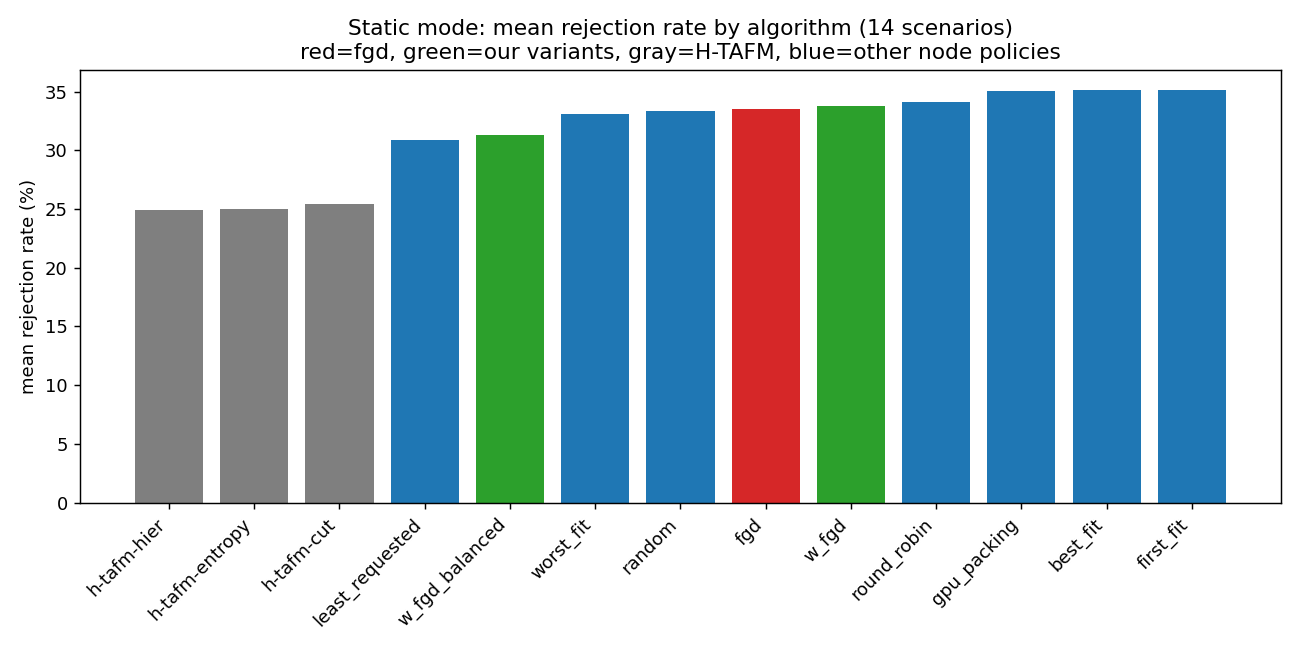
\includegraphics[width=0.8\textwidth]{../../experiments/runs/2026-09-12_fgd_vs_wfgd_htafm/plots/01_static_rejection_by_algorithm.png}
\caption{Mean rejection rate by algorithm, static mode, averaged over 14 scenarios.}
\label{fig:static-rejection}
\end{figure}

\begin{figure}[h]
\centering
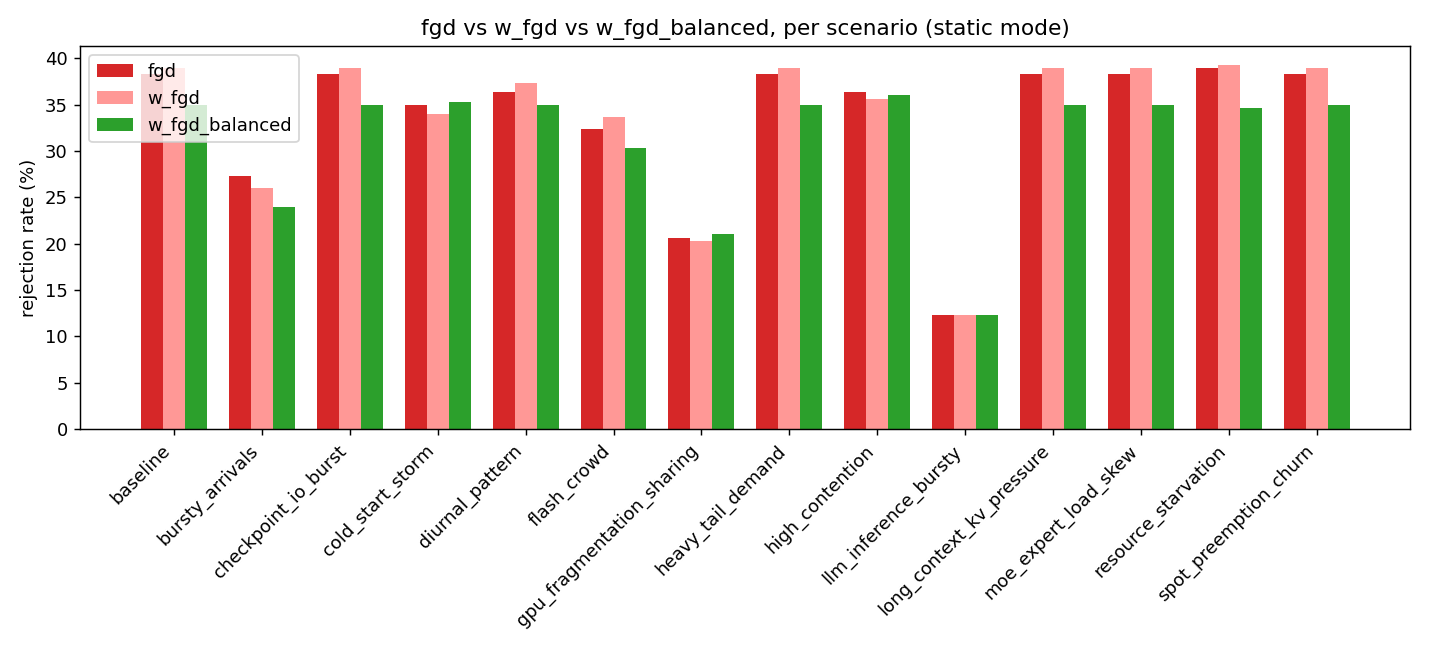
\includegraphics[width=0.85\textwidth]{../../experiments/runs/2026-09-12_fgd_vs_wfgd_htafm/plots/02_fgd_vs_wfgd_per_scenario.png}
\caption{fgd vs. w\_fgd vs. w\_fgd\_balanced, paired per scenario.}
\label{fig:fgd-comparison}
\end{figure}

\begin{figure}[h]
\centering
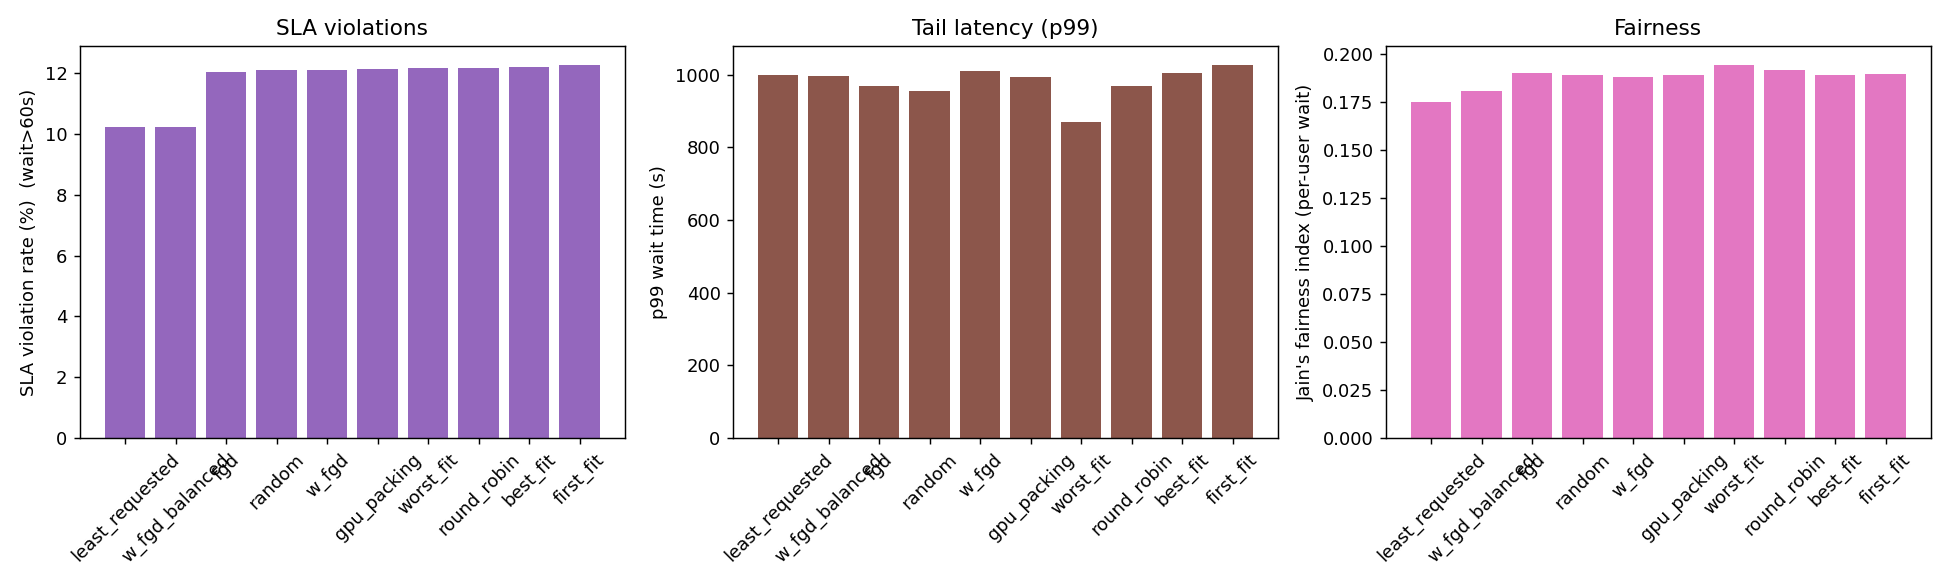
\includegraphics[width=\textwidth]{../../experiments/runs/2026-09-12_fgd_vs_wfgd_htafm/plots/03_broader_metrics_comparison.png}
\caption{SLA violation rate, p99 tail latency, and Jain's fairness index, time-driven mode.}
\label{fig:broader}
\end{figure}

\begin{figure}[h]
\centering
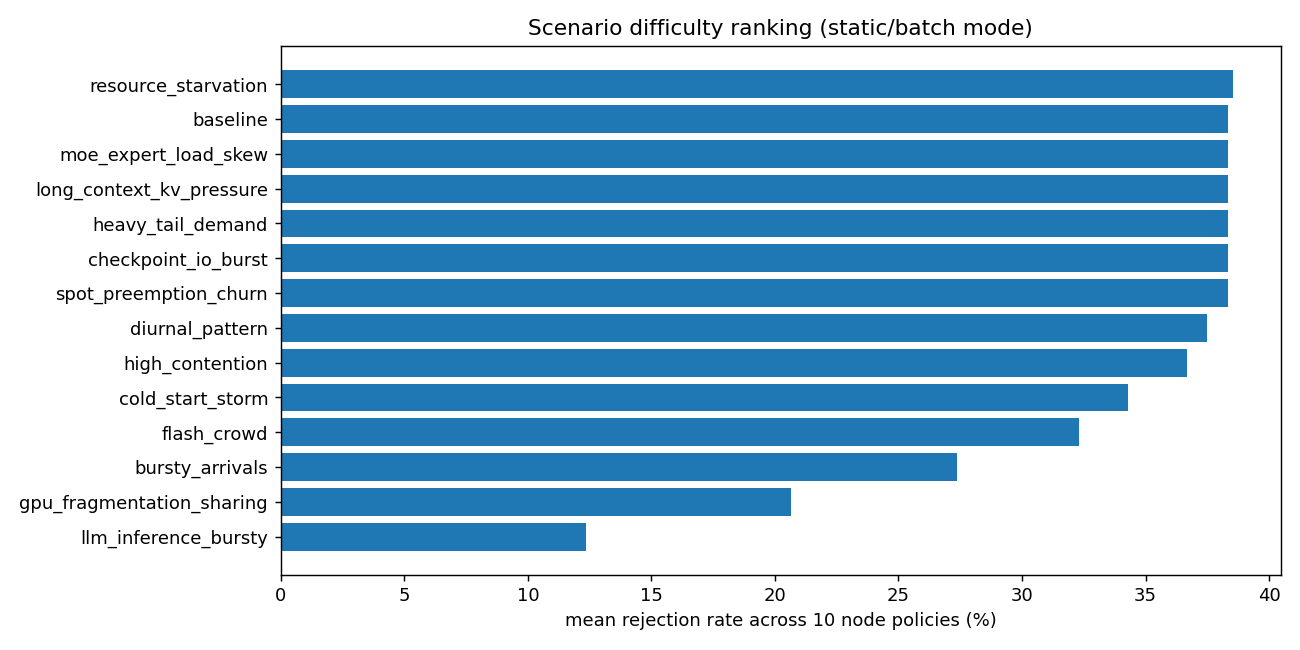
\includegraphics[width=0.8\textwidth]{../../experiments/runs/2026-09-12_fgd_vs_wfgd_htafm/plots/04_scenario_difficulty.png}
\caption{Scenario difficulty ranking, static mode.}
\label{fig:scenario-diff}
\end{figure}

% =====================================================================
\section{Discussion and Limitations}
% =====================================================================
\begin{enumerate}[leftmargin=1.4em]
\item \textbf{H-TAFM's static-mode advantage is confounded by granularity
  and a synthetic memory dimension} (\S\ref{sec:mem-assumption}). We
  cannot separate ``the delta-TAFI heuristic is better'' from ``NUMA-vertex
  splitting mechanically eases bin-packing'' from these results alone.
\item \textbf{Significance at this scale (300 jobs/scenario) does not
  guarantee significance at production scale.} Rejection-rate differences
  are highly significant; time-driven wait-time/fairness differences are
  mostly not, at this specific contention level (\S\ref{sec:broader-metrics}).
  Both are honestly reported rather than the more favorable one only.
\item \textbf{$\lambda=0.15$ is tuned, not derived.} Section~\ref{sec:wfgd}.
\item \textbf{The \texttt{heavy\_tail\_demand} discrepancy}
  (\S\ref{sec:scenarios}) means any result specific to that scenario in
  this document should be read as ``baseline, relabeled,'' not as evidence
  about heavy-tailed demand specifically, until fixed upstream.
\end{enumerate}

% =====================================================================
\section{Conclusion}
% =====================================================================
\textsc{w-fgd-balanced} is a small, precisely-motivated modification of
FGD (real, weighted representative shapes; a slack-preservation
regularizer) that produces a statistically significant, if modest,
improvement over FGD specifically, matches (does not exceed) the
strongest simple existing baseline, and its H-TAFM comparison should be
read with the granularity and memory-assumption caveats above firmly
attached. All numbers reproduce from the archived checkpoint described in
\S\ref{sec:repro}.

\begin{thebibliography}{9}
\bibitem{fgd} Weng et al., ``Beware of Fragmentation: Scheduling
  GPU-Sharing Workloads with Fragmentation Gradient Descent,'' USENIX ATC 2023.
\bibitem{defrag} Mishra \& Bellur, ``De-Fragmenting the Cloud,'' arXiv:1506.07020, 2015.
\bibitem{hypergraph_survey} Wang \& Wu, ``Survey on Hypergraph Algorithms
  ... in Cloud Computing,'' J. Comput. Sci. Technol. 41(2), 2026.
\bibitem{partitioning_hard} Papp, Anegg, Yzelman, ``Partitioning
  Hypergraphs is Hard,'' SPAA 2023.
\bibitem{binpacking_survey} Christensen et al., ``Multidimensional Bin
  Packing and Other Related Problems: A Survey,'' 2016.
\bibitem{jain1984} Jain, Chiu \& Hawe, ``A Quantitative Measure Of Fairness
  And Discrimination For Resource Allocation In Shared Computer Systems,''
  DEC Research Report TR-301, 1984.
\end{thebibliography}

\end{document}
